\chapter{Frontend Implementation}

\section{Technology Stack}

The frontend of Campus-Sync is built using modern web technologies that provide a responsive, performant, and maintainable user interface:

\begin{itemize}
    \item \textbf{React 18}: A JavaScript library for building user interfaces with component-based architecture
    \item \textbf{TypeScript}: A typed superset of JavaScript that compiles to plain JavaScript
    \item \textbf{Vite}: A next-generation frontend tooling that provides fast development and build processes
    \item \textbf{Tailwind CSS}: A utility-first CSS framework for rapidly building custom user interfaces
    \item \textbf{shadcn/ui}: A collection of accessible, customizable UI components built with Radix UI and Tailwind CSS
    \item \textbf{React Router v6}: Declarative routing for React applications
    \item \textbf{React Hook Form}: Performant, flexible forms with easy validation
    \item \textbf{Zod}: TypeScript-first schema declaration and validation library
    \item \textbf{Recharts}: A composable charting library built on React components
    \item \textbf{Lucide React}: A library of simply beautiful open source icons
\end{itemize}

\section{Component Architecture}

The frontend follows a modular component architecture with clear separation of concerns. Components are organized in a hierarchical structure:

\subsection{Component Hierarchy}

\begin{figure}[H]
    \centering
    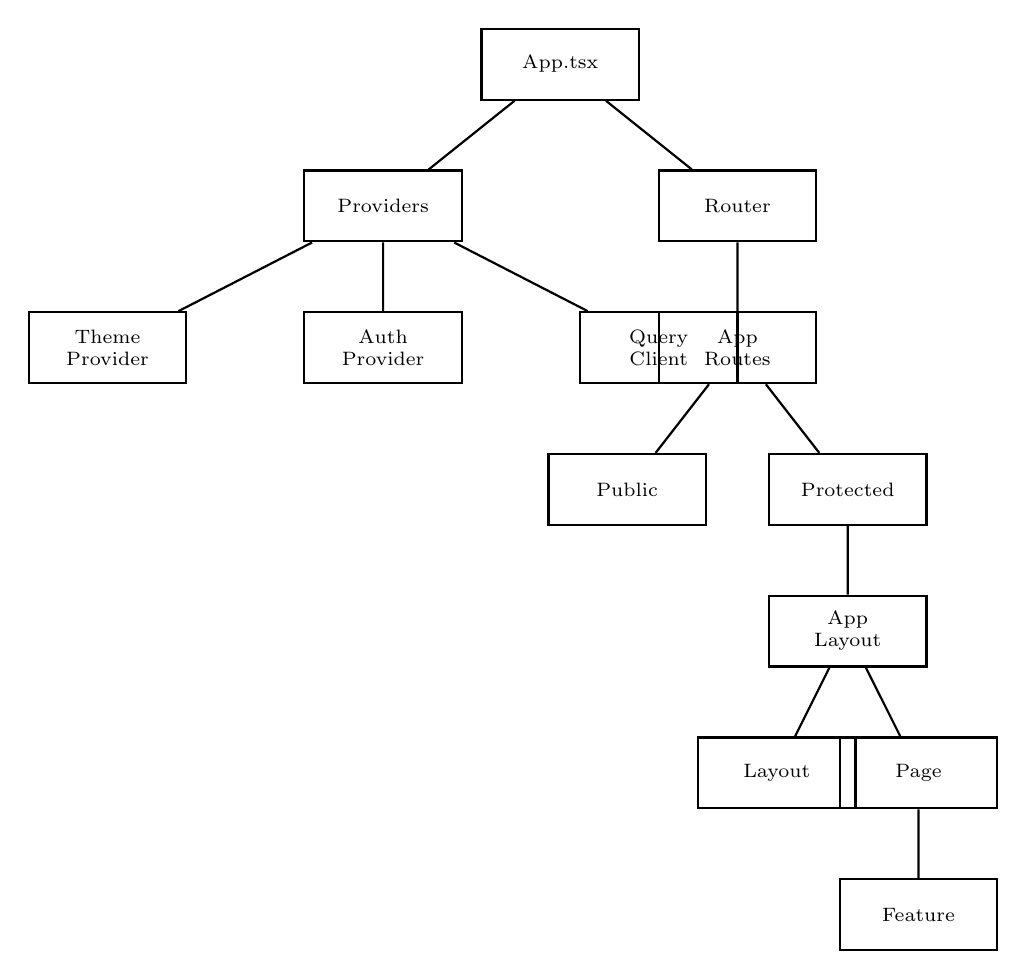
\begin{tikzpicture}[thick, level distance=1.8cm,
      level 1/.style={sibling distance=4.5cm},
      level 2/.style={sibling distance=3.5cm},
      level 3/.style={sibling distance=2.8cm},
      level 4/.style={sibling distance=2.2cm},
      level 5/.style={sibling distance=1.8cm},
      level 6/.style={sibling distance=1.5cm},
      every node/.style={align=center, rectangle, draw, minimum width=2cm, minimum height=0.9cm, font=\scriptsize}]
      \node {App.tsx}
        child { node {Providers}
          child { node {Theme\\Provider} }
          child { node {Auth\\Provider} }
          child { node {Query\\Client} }
        }
        child { node {Router}
          child { node {App\\Routes}
            child { node {Public} }
            child { node {Protected}
              child { node {App\\Layout}
                child { node {Layout} }
                child { node {Page}
                  child { node {Feature} }
                }
              }
            }
          }
        };
    \end{tikzpicture}
    \caption{Component Hierarchy Tree}
    \label{fig:component-hierarchy}
\end{figure}

\subsection{Folder Structure}

The frontend codebase is organized into the following directory structure:

\begin{verbatim}
src/
├── assets/               # Static assets (images, icons, etc.)
├── components/           # Reusable UI components
│   ├── about/            # About page components
│   ├── admin/            # Admin-specific components
│   ├── announcements/    # Announcement components
│   ├── assignments/      # Assignment components
│   ├── attendance/       # Attendance components
│   ├── auth/             # Authentication components
│   ├── billing/          # Billing components
│   ├── calculators/      # Calculator components
│   ├── community/        # Community components
│   ├── courses/          # Course components
│   ├── dashboard/        # Dashboard components
│   ├── exams/            # Exam components
│   ├── expenses/         # Expense components
│   ├── features/         # Feature components
│   ├── fitness/          # Fitness components
│   ├── layout/           # Layout components
│   ├── marks/            # Marks components
│   ├── meditation/       # Meditation components
│   ├── music/            # Music components
│   ├── mycourses/        # My courses components
│   ├── notes/            # Notes components
│   ├── profile/          # Profile components
│   ├── shared/           # Shared components
│   ├── students/         # Student components
│   ├── ui/               # Base UI components (shadcn/ui)
│   ├── ProtectedRoute.tsx # Route protection component
│   ├── PublicRoute.tsx    # Public route component
│   ├── RoleRoute.tsx      # Role-based route component
│   ├── SEO.tsx           # SEO component
│   ├── ScrollToTop.tsx   # Scroll to top component
│   ├── app-sidebar.tsx   # Application sidebar
│   ├── nav-main.tsx      # Main navigation
│   ├── nav-projects.tsx  # Projects navigation
│   ├── nav-secondary.tsx # Secondary navigation
│   ├── nav-user.tsx      # User navigation
│   ├── theme-provider.tsx # Theme provider
│   └── theme-toggle.tsx  # Theme toggle
├── contexts/             # React context providers
│   └── AuthContext.tsx   # Authentication context
├── data/                 # Static data files
│   └── courseData.ts     # Course data
├── hooks/                # Custom React hooks
│   ├── index.ts          # Hooks exports
│   ├── use-mobile.tsx    # Mobile detection hook
│   ├── use-page-loading.tsx # Page loading hook
│   ├── use-toast.ts      # Toast notification hook
│   ├── useAdminData.ts   # Admin data hook
│   ├── useAdminIDData.ts # Admin ID data hook
│   ├── useAudioPlayer.ts # Audio player hook
│   ├── useLocalStorage.ts # Local storage hook
│   ├── useSEO.ts         # SEO hook
│   ├── useStudentIDData.ts # Student ID data hook
│   ├── useTeacherIDData.ts # Teacher ID data hook
│   └── useUserData.ts    # User data hook
├── lib/                  # Utility libraries
│   ├── index.ts          # Library exports
│   └── utils.ts          # Utility functions
├── pages/                # Page components
│   ├── admin/            # Admin pages
│   ├── student/          # Student pages
│   ├── teacher/          # Teacher pages
│   └── shared/           # Shared pages
├── routes/               # Route definitions
│   ├── admin/            # Admin routes
│   ├── student/          # Student routes
│   ├── teacher/          # Teacher routes
│   ├── common/           # Common routes
│   ├── AppRoutes.tsx     # Main routes
│   ├── ProtectedRoutes.tsx # Protected routes
│   ├── PublicRoutes.tsx  # Public routes
│   └── index.ts          # Routes exports
├── types/                # TypeScript types
│   ├── academic.ts       # Academic types
│   ├── attendance.ts     # Attendance types
│   └── exam.ts           # Exam types
├── App.css               # Global styles
├── App.tsx               # Main application component
├── index.css             # Base styles
├── main.tsx              # Application entry point
└── vite-env.d.ts         # Vite environment types
\end{verbatim}

\section{State Management}

Campus-Sync employs multiple state management strategies depending on the scope and nature of the data:

\subsection{Context API}

The Context API is used for global state management, particularly for authentication and theming:

\begin{itemize}
    \item \textbf{AuthContext}: Manages user authentication state, including login status, user role, and profile information
    \item \textbf{ThemeContext}: Handles dark/light mode preferences and theme-related state
\end{itemize}

\subsection{Custom Hooks}

Custom hooks encapsulate reusable logic and state management patterns:

\begin{itemize}
    \item \textbf{useAuth}: Provides authentication state and methods
    \item \textbf{useUserData}: Manages user-specific data fetching and caching
    \item \textbf{useLocalStorage}: Handles persistent storage in the browser's local storage
    \item \textbf{useMobile}: Detects mobile device usage for responsive design
    \item \textbf{useSEO}: Manages SEO metadata for pages
\end{itemize}

\subsection{React Query}

React Query is used for server state management, providing:

\begin{itemize}
    \item Data caching and synchronization
    \item Background data fetching
    \item Mutation handling
    \item Pagination support
\end{itemize}

\section{Routing Structure}

The application implements a comprehensive routing system with role-based access control:

\subsection{Route Organization}

\begin{itemize}
    \item \textbf{Public Routes}: Authentication pages accessible to all users
    \item \textbf{Protected Routes}: Application features requiring authentication
    \item \textbf{Role Routes}: Panel-specific routes for students, teachers, and administrators
    \item \textbf{Common Routes}: Shared features accessible to all authenticated users
\end{itemize}

\subsection{Navigation Structure}

The navigation system includes:

\begin{itemize}
    \item Main sidebar navigation with role-specific items
    \item Breadcrumb navigation for context awareness
    \item Quick access toolbar for frequently used features
\end{itemize}

\section{UI/UX Design}

The user interface follows modern design principles to ensure an intuitive and engaging user experience.

\subsection{Design System}

\begin{itemize}
    \item \textbf{Color Palette}: Primary, Secondary, Success, Warning, Error, and Neutral colors
    \item \textbf{Typography}: Responsive font sizing with consistent hierarchy
    \item \textbf{Spacing}: 8px base unit with consistent spacing scale
    \item \textbf{Breakpoints}: Mobile (320px), Tablet (768px), Desktop (1024px), Large Desktop (1440px)
\end{itemize}

\subsection{Responsive Design}

\begin{itemize}
    \item Mobile-first approach
    \item Flexible grid system
    \item Touch-friendly interactions
    \item Adaptive layouts for different screen sizes
\end{itemize}

\subsection{Accessibility}

\begin{itemize}
    \item WCAG 2.1 AA compliance
    \item Semantic HTML structure
    \item Keyboard navigation support
    \item Screen reader compatibility
    \item Proper contrast ratios
\end{itemize}

\section{Performance Optimization}

Several optimization techniques are implemented to ensure fast loading and smooth interactions:

\subsection{Code Splitting}

\begin{itemize}
    \item Route-based code splitting
    \item Dynamic imports for heavy components
    \item Lazy loading of non-critical features
\end{itemize}

\subsection{Bundle Optimization}

\begin{itemize}
    \item Tree shaking for unused code
    \item Minification and compression
    \item Image optimization
    \item Font loading optimization
\end{itemize}

\subsection{Caching Strategy}

\begin{itemize}
    \item Browser caching for static assets
    \item Service worker for offline support
    \item React Query caching for API responses
    \item Local storage for user preferences
\end{itemize}

\section{Authentication and Authorization}

The authentication system implements JWT-based security with role-based access control:

\subsection{Authentication Flow}

\begin{enumerate}
    \item User visits authentication page
    \item Credentials submitted to backend
    \item JWT tokens received and stored
    \item User redirected to appropriate dashboard
    \item Tokens refreshed automatically before expiry
\end{enumerate}

\subsection{Role-Based Access Control}

\begin{itemize}
    \item \textbf{Student}: Access to student dashboard, courses, assignments, grades
    \item \textbf{Teacher}: Access to teacher dashboard, class management, grading
    \item \textbf{Admin}: Access to admin dashboard, user management, system settings
\end{itemize}

This frontend implementation provides a solid foundation for the Campus-Sync platform, ensuring a responsive, accessible, and performant user experience across all devices and user roles.